% Generated by analyse_t_mode_consistency.py.
\textbf{Used impedance.} The gains in the surface basis $[t_1,t_2,n]$ are
\begin{align*}
K_p&=[2000,2000,1000]\,\mathrm{N/m}, &
K_R&=[15,5,50]\,\mathrm{N\,m/rad},\\
D_p&=[10.00,10.00,175.00]\,\mathrm{N\,s/m}, &
D_R&=[10.010,10.010,10.000]\,\mathrm{N\,m\,s/rad}.
\end{align*}
The centre of compliance is at the TCP, $r_c=0$. The grey areas mark the stationary intervals: 8--13\,s for $F_n$ and 28.5--31\,s for $M_{t_1}$. The measured means are calculated only from these intervals.

\begin{center}
  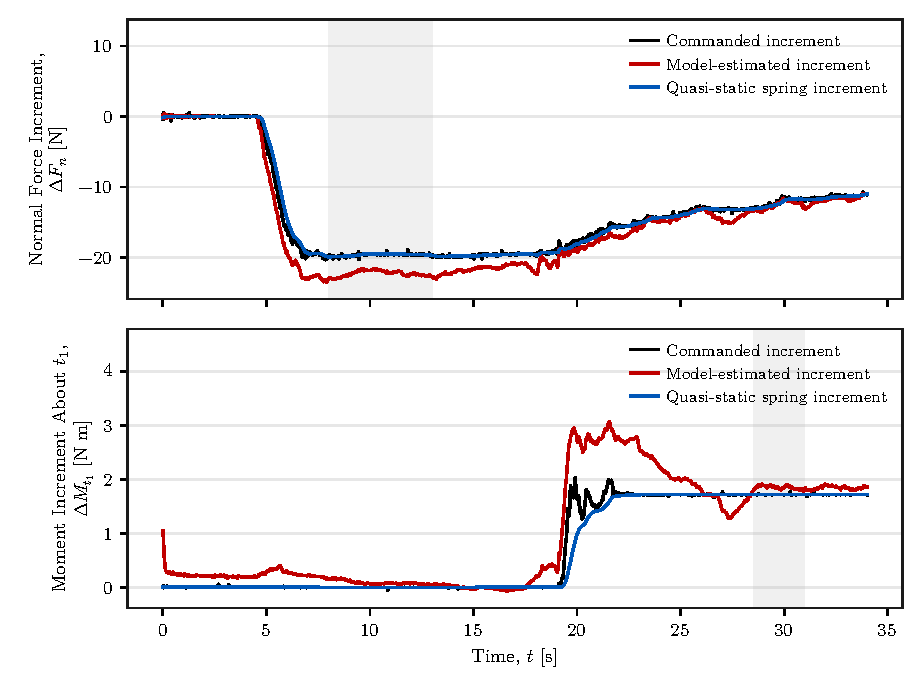
\includegraphics[width=0.92\textwidth]{professoremail/t_mode_consistency.pdf}
\end{center}

\begin{center}
\scriptsize
\begin{tabular}{lrrrrl}
\hline
Component & Achieved & Quasi-static & Commanded & Estimated & Status \\
\hline
$F_n$ & -19.65 mm & -19.650 & -19.640 & -22.292 & consistent \\
$M_{t_1}$ & 6.565 deg & 1.719 & 1.719 & 1.852 & consistent \\
\hline
\end{tabular}
\end{center}



\textbf{Normal force $F_n$.}
\[
F_{n,\mathrm{qs}}=K_{p,n}\mathbin{\cdot}e_n
=1000\mathbin{\cdot}(-0.019650)=-19.650\,\mathrm{N}.
\]
The commanded mean is $-19.640\,\mathrm{N}$.  The quasi-static difference is $0.010\,\mathrm{N}$ (0.05\%).  The model-estimated mean is $-22.292\,\mathrm{N}$, a difference of $2.652\,\mathrm{N}$ (13.50\%).

\textbf{Moment $M_{t_1}$.}
\[
M_{t_1,\mathrm{qs}}=K_{R,t_1}\mathbin{\cdot}e_{R,t_1}
=15\mathbin{\cdot}(6.565\pi/180)=1.719\,\mathrm{N\,m}.
\]
The commanded mean is $1.719\,\mathrm{N\,m}$.  The quasi-static difference is $0.000\,\mathrm{N\,m}$ (0.00\%).  The model-estimated mean is $1.852\,\mathrm{N\,m}$, a difference of $0.133\,\mathrm{N\,m}$ (7.75\%).
